\documentclass[a4paper,12pt]{article}

%%% Работа с картинками
\usepackage{wrapfig} % Обтекание рисунков и таблиц текстом

%%% Работа с русским языком
\usepackage{cmap}					% поиск в PDF
\usepackage{mathtext} 				% русские буквы в фомулах
\usepackage[T2A]{fontenc}			% кодировка
\usepackage[utf8]{inputenc}			% кодировка исходного текста
\usepackage[russian]{babel}	% локализация и переносы

%%% Дополнительная работа с математикой
\usepackage{amsmath,amsfonts,amssymb,amsthm,mathtools} % AMS
\usepackage{icomma} % "Умная" запятая: $0,2$ --- число, $0, 2$ --- перечисление

\usepackage{multirow}
\usepackage{physics}
\usepackage{cite}
\usepackage{setspace}
\usepackage{xcolor}
\usepackage[hidelinks,pagebackref=false,pdfnewwindow=true]{hyperref}
\usepackage{xcolor}
\definecolor{linkcolor}{cmyk}{1,0.7,0,0}
\definecolor{urlcolor}{cmyk}{1,0.7,0,0}



%% Номера формул
\mathtoolsset{showonlyrefs=true} % Показывать номера только у тех формул, на которые есть \eqref{} в тексте.

%% Шрифты
\usepackage{euscript}	 % Шрифт Евклид
\usepackage{mathrsfs} % Красивый матшрифт
\usepackage{fancyhdr}

%% Работа с гиперссылками
\usepackage{xcolor}
\usepackage{hyperref}
% Цвета для гиперссылок
\definecolor{linkcolor}{HTML}{799B03} % цвет ссылок
\definecolor{urlcolor}{HTML}{799B03} % цвет гиперссылок
\hypersetup{pdfstartview=FitH,  linkcolor=linkcolor,urlcolor=urlcolor, colorlinks=true}

%% Работа с картинками
\usepackage{graphicx}
\usepackage{caption}
\usepackage{subcaption}
\graphicspath{{pictures/}}
\DeclareGraphicsExtensions{.pdf,.png,.jpg,.eps}

%% Геометрия и отступы
\usepackage[hmarginratio=1:1,top=32mm, headheight=16pt]{geometry}
\pagestyle{empty}
\usepackage{floatrow}

%% Свои команды
\pagenumbering{arabic}

\begin{document} % конец преамбулы, начало документа

\begin{center}
	\vspace{5ex}
	\textbf{ФЕДЕРАЛЬНОЕ ГОСУДАРСТВЕННОЕ АВТОНОМНОЕ ОБРАЗОВАТЕЛЬНОЕ }\\
	\textbf{ УЧРЕЖДЕНИЕ ВЫСШЕГО ОБРАЗОВАНИЯ }\\
	\textbf{ <<НАЦИОНАЛЬНЫЙ ИССЛЕДОВАТЕЛЬСКИЙ УНИВЕРСИТЕТ }\\
	\textbf{ <<ВЫСШАЯ ШКОЛА ЭКОНОМИКИ>>}\\
	\vspace{5ex}
	Факультет физики\\
	\vspace{5ex}
	\textbf{Кравцов Михаил Викторович}\\
	\vspace{3ex}
	\Large{\textbf{Спиновая когерентность электронов в ионах $Ce^{3+}$,}\\
	\textbf{встроенных в кристалл YAG }}\\
	\vspace{3ex}
	Выпускная квалификационная работа\\
	по направлению подготовки 03.03.02 Физика\\
	образовательная программа «Физика»\\
	\par\end{center}

\vspace{17ex}

\noindent \begin{flushright}
	Научный руководитель\\
	к.ф.-м.н., с.н.с., ФИАН \\
	Белых Василий Валерьевич\\
	
	\par\end{flushright}

\begin{center}
	\vfill{}
	Москва 2022
	\par\end{center}

\thispagestyle{empty}

\newpage

\section{Аннотация}
\large{
Изучение спиновой динамики в полупроводниках во внешнем магнитном поле сталквается с проблемой рассинхронизации прецессии спинов, связанной с различными взаимодействиями в спиновом ансамбле. Различия частот прецессии микроскопических спинов достигается не только за счет Зеемановского расщепления, но также за счет спин-орбитального взаимодействия, взаимодействия с эффективным полем ядерных спинов, спин-фононных, электрон-дырочных и электрон-электронных взаимодействий. \\
Для синхронизации спинового ансамбля применяются различные методы, в числе которых приложения радиочастотного поля (рч), ортогонального направлению внешнего магнитного поля. При совпадении переменного рч-поля с Ларморовской частотой прецессии в магнитном поле, в образцах может наблюдаться электронный парамагнитный резонанс (ЭПР). В данной реализации ЭПР микроскопические спины в ансамбле синхронизированы и прецессируют когерентно, становясь отвязанными от меняющихся во времени внешних неоднородностей. Так, когерентный макроскопический спиновый ансамбль может быть детектирован поворотом плоскости поляризации линейно поляризованного света.\\
При помощи накачки электронов в зону проводимости циркулярно поляризованными лазерными импульсами, можно также добиться когерентного вращения спинов в ансамбле. \\
Если частота накачки импульсами лазера будет совпадать с Ларморовской частотой прецесии и частотой РЧ поля, то в системе будет реализовано, так называемое, стимулированное резонансное спиновое усиление. Данный метод позволяет отедлить спиновый ансамбль не только от влияния быстро меняющегося во времени неоднородного окружения, но также отвязать ее от влияния эффективного поля, создаваемого ядерными спинами. Таким образом, в данной постановке эксперимента измеряется время спиновой когерентности $T_2$, а также появляется возможность изучения влияния внешнего радиочастотного поля на спиновую когерентность.\\
Исследуя поведение спинового ансамбля в переменном РЧ поле в образце YAG (иттрий-алюминиевого граната), нами было получено время спиновой когерентности порядка 1 мс, получено следствие того, что ансамбль <<не забывает>> предыдущее воздействие РЧ поля на временах порядка $T_2$. Была исследована зависимость времени спиновой когерентности от параметра скважности - доли РЧ поля в периоде радиочастотной модуляции. Результатами данных исследований стало то, что максимальная степень синхронизации микрокопических спинов в ансамбле достигается при 70\%-ной доле РЧ воздействия в периоде модуляции и что в отсутствии переменного поля время спиновой когерентности ансамбля было выше, чем при наличии РЧ поля.}
\newpage

\tableofcontents
\newpage

\section{Введение}
Исследование спиновой динамики электронов представляет существенный фундаментальный и практический интерес. Электрон, являясь двухуровневой системой, может быть использован для создания квантового бита - кубита. Кубит характеризуется двумя собственными значениями |0> и |1>, а также их суперпозицией A|0> + B|1>, где $A$ и $B$ - Амплитуды вероятности соответствующих значений. Также как и состояние кубита, поляризацию спина удобно представить на сфере Блоха:

\begin{wrapfigure}{o}{0.5\linewidth}
	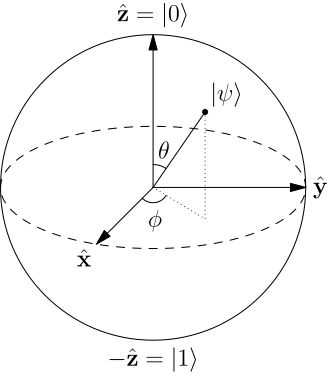
\includegraphics[scale = 0.4]{Bloch.png}
	\caption{\textit{Сфера Блоха для состояния кубита и поляризации спина. Амплитуды вероятностей собственных значений кубита |0> и |1> соответственно $A = \cos{\frac{\Theta}{2}}$, $B = e^{i \phi} \sin{\frac{\Theta}{2}}$}}
		\label{fig:Bloch}
\end{wrapfigure}

Таким образом, пространственное положение спина, характеризующееся полярным углом $\phi$ и азимутальным углом $\theta$ задает амплитуды вероятности кубита $A$ и $B$ оказаться в одном из двух его собственных значений. \\

В классическом представлении спину электрона соответствует его механический момент импульса. Электрон, являясь заряженной частицей, обладает магнитным моментом $\frac{g \mu_b}{2}$, где g-фактор связывает магнитный момент и момент импульса, в следствии чего электрон прецессирует вокруг направления магнитного поля. Время $T_2$ характеризует способность спина возвращаться в изначальное равновесное состояние после возбуждения. Данное равновесное состояние достигается, когда спин будет ориентирован по полю.\\
Одной из важнейших задач спиновой физики является не только поиск материалов с длинным временем спиновой релаксации, но и поиск способов манипулирования спиновым ансамблем для повышения времени спиновой когерентности $T_2$, отражающим способность системы релаксировать во внешнем магнитном поле. \\

В присутствии поля $B$ вырождение энергетических уровней спиновых состояний с $S = \pm \frac{1}{2}$ снимается Зеемановским расщеплением 
\begin{equation}\label{dE}
\Delta E = 2 \pi \hbar f_L 
\end{equation}
где $f_L$ - Ларморовская частота $f_L = \frac{g \mu_b B}{2 \pi \hbar}$. Тензор g-фактора определяет частоту и направление прецессии спина во внешнем магнитном поле. \\
Когерентность данной прецессии определяется временем $T_2$, которое и исследуется в нашей работе для системы редкоземельных ионов $Ce^{3+}$ в решетке итрий-алюминиевого граната YAG. \\

В свою очередь, переворот спина, направленного вдоль магнитного поля происходит за время $T_1$, которое называется временем продольной спиновой релаксации. Во время релаксации, электрон переходит с верхнего энергетического уровня на нижний, что требует диссипации энергии, которая зачастую испускается в виде акустического фонона. \\
Времена релаксации $T_1$ и $T_2$ определяют затухание продольной и поперечной компоненты спина соответственно. \\

Большое количество экспериментов по изучению спиновой динамики и, в частности, времени спиновой когерентности $T_2$ сталкивается с неоднородностями в спиновом ансамбле, вносящими вклад, быстро меняющийся по времени. Таким образом, спиновая когерентность ограничена не временем $T_2$, характерным для самой системы, а эффективным временем изменения окружения ансамбля и расфокусировкой микроскопических спинов, связанной с дисперсией Ларморовских частот и эффективным полем ядерных спинов.

\begin{figure}[h!]
	\centering
	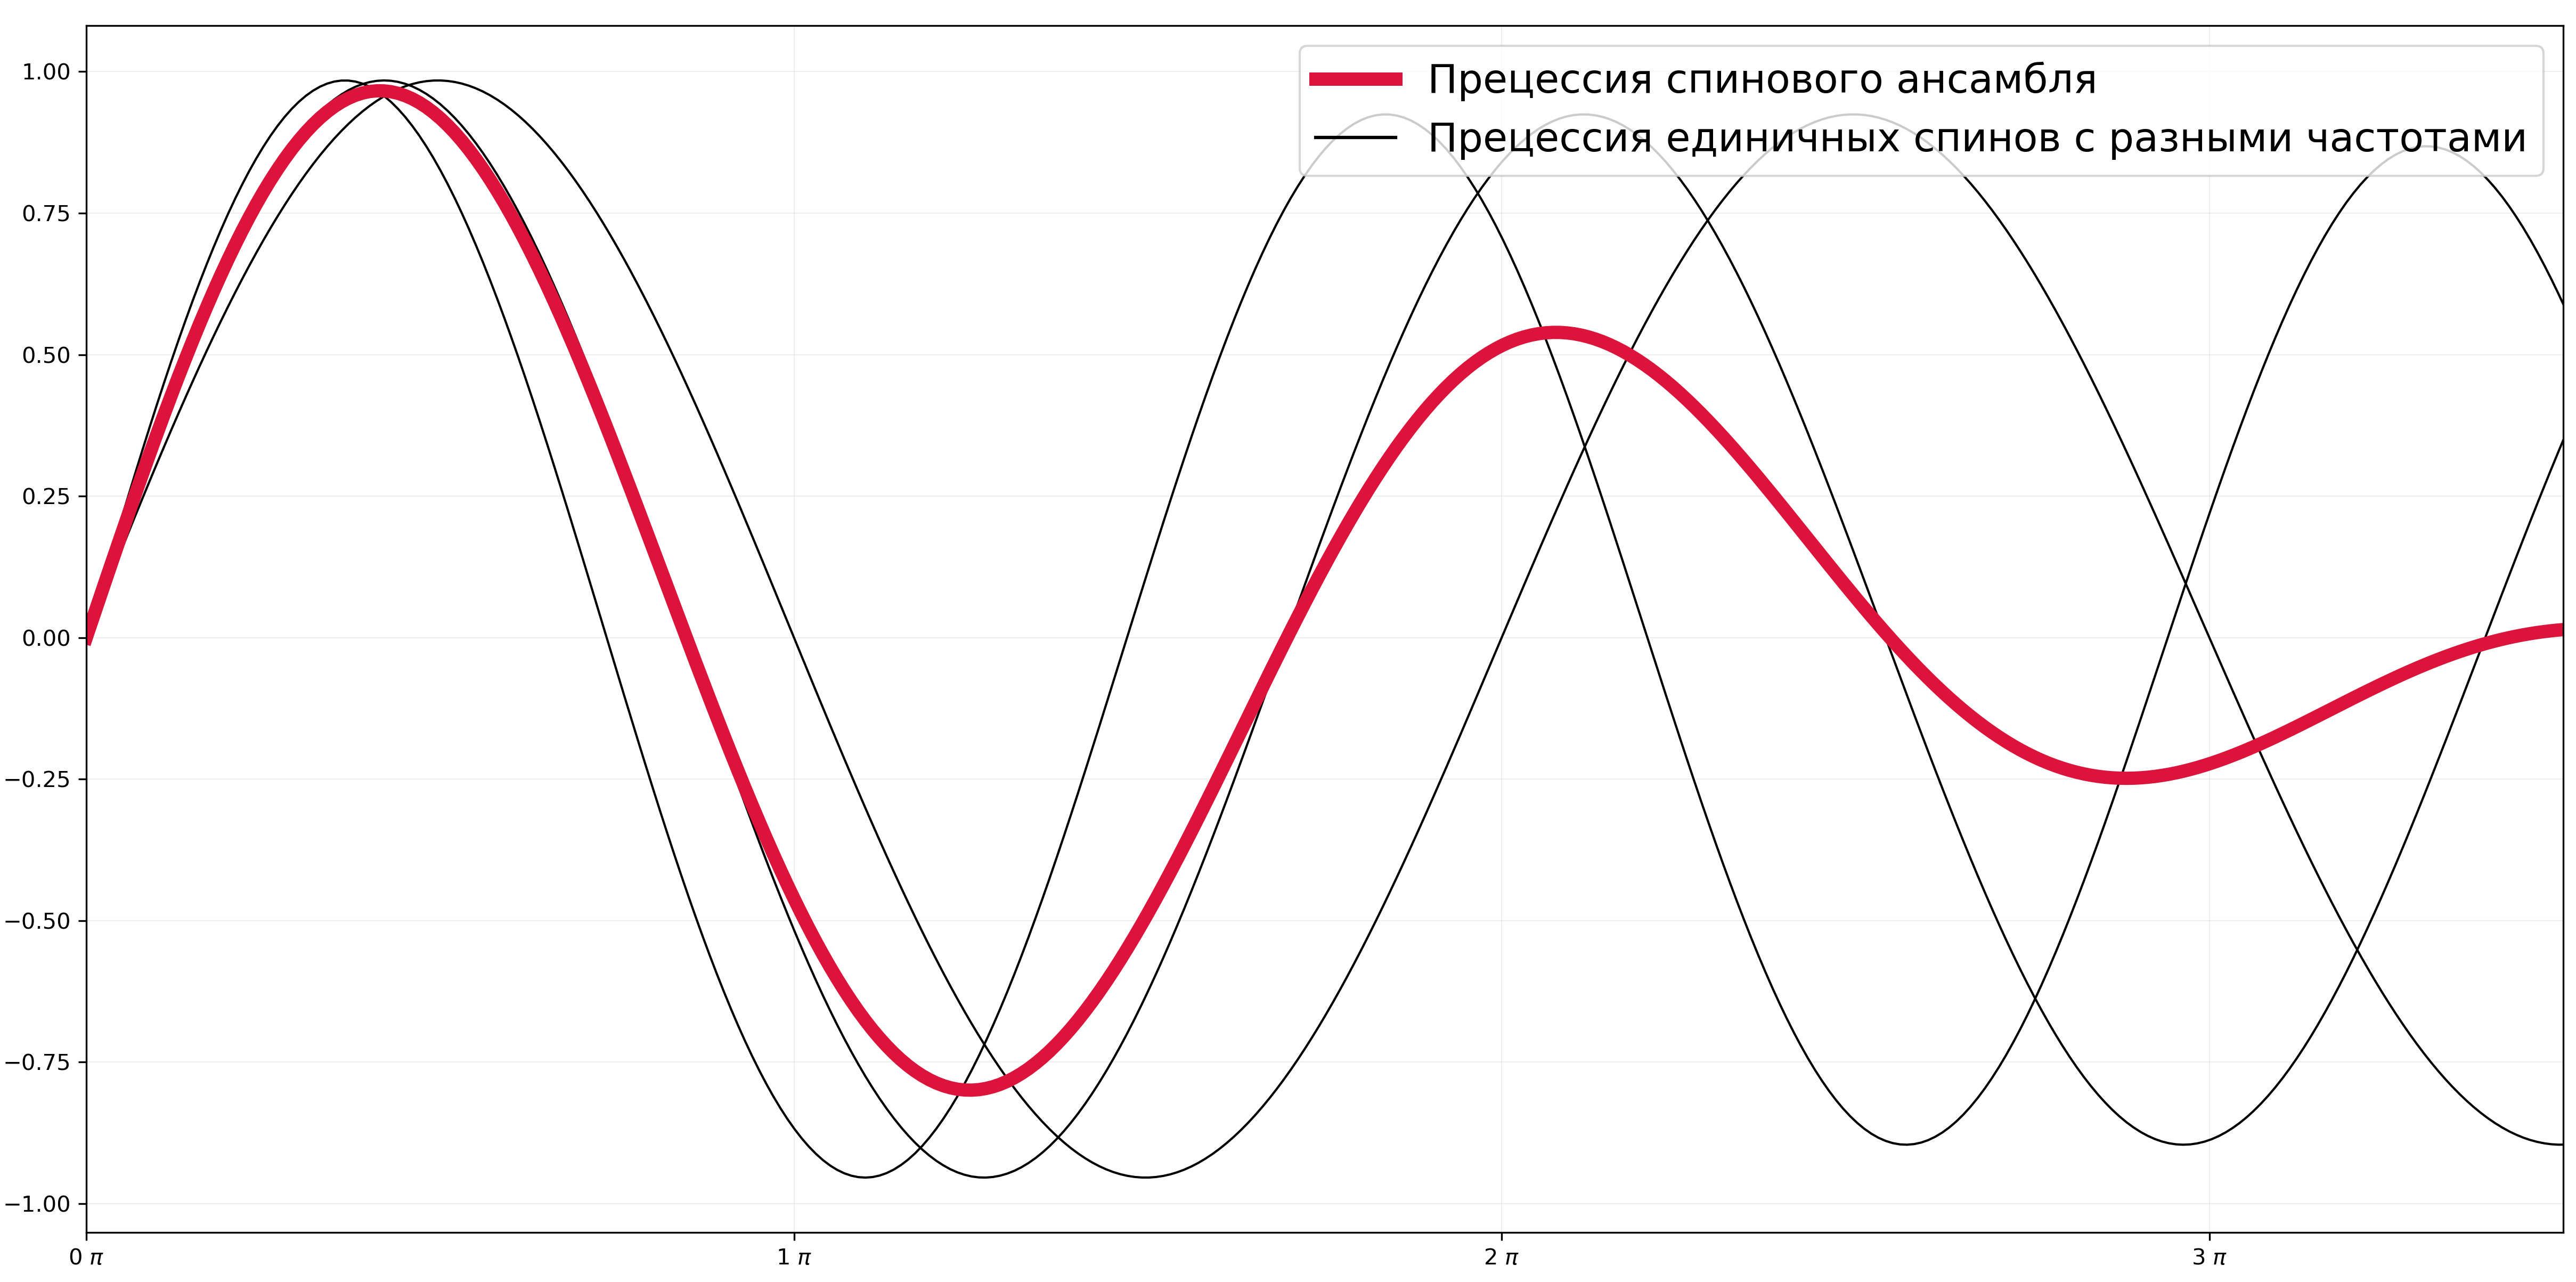
\includegraphics[scale = 0.17]{inh.png}
	\caption{\textit{Прецессия индивидуальных спинов (черные кривые)
			и макроскопического спина в ансамбле (красная кривая). Когерентность ансамбля длится меньше, чем когерентность единичного спина}}
	\label{fig:inh}
\end{figure}

Ансамбль спинов теряет макроскопическую спиновую когерентность гораздо быстрее, чем индивидуальный спин. Эффект расфокусировки индивидуальных спинов приводит к запаздыванию или опережению прецессии одних спинов относительно других внутри ансамбля. Несмотря на то, что каждый единичный спин сохраняет свою когерентность, ансамбль её теряет в результате быстрой фазовой расстройки. \\
Когерентность спинового ансамбля характеризуется временем $T_2^*$, называемым временем спиновой дефазировки. Время $T_2^* < T_2$ и именно оно определяет ширину резонанса ЭПР и резонансного спинового усиления\cite{kikkawa}. \\

При приложении к спиновому ансамблю переменного радиочастотного поля с частотой, совпадающей с Ларморовской $f_L$, микроскопические спины синхронизируются под действием внешнего возбуждения и <<отвязываются>> от быстро меняющегося неоднородного окружения. Данный эффект усиливается воздействием периодических циркулярно поляризованных лаерных импульсов, накачивающих электроны в зону проводимости. Таким образом, чтобы изолировать систему от влияния неоднородностей, в нашей работе применено сочетание электронного парамагнитного резонанса и резонансного спинового усиления, когда частота РЧ поля, частота оптических импульсов и Ларморовская частота равны $f_{rf} = f_o = f_L$. Данный подход называется стимулированное резонансное спиновое усиление и позволяет напрямую измерять время $T_2 \approx T_2^*$ без учета воздействия неоднородностей и ядерных спинов на ансамбль. \\

В данной работе рассмотрена экспериментальная реализация стимулированного резонансного спинового усиления, при помощи которой произведено манипулирование спиновым ансамблем для исследования зависимости времени спиновой когерентности $T_2$ от парметров РЧ поля. 

\section{Литературный обзор}

Бурное развитие спинтроники и приложений к созданию квантовых компьютеров потребовало как можно более локальных и быстрых методов взаимодействия и манипулирования спиновыми системами. Таким образом, использование классических методов наряду с оптическими привело к развитию и дальнейшему совершенствованию последних.\\
Впервые опыты по оптическому возбуждению и детектированию оптической ориентации в атомах были проведены в парах ртути \cite{mercury} Кастлером и Бросселем. Оптическая накачка электронов со спиновой поляризацией циркулярно поляризованным светом была же впервые реализована в твердых телах в изотопе кремния $Si^{29}$ \cite{silicium}. \\
Затухание поперечной компоненты спина длится в течении $T_2$, которое также называется временем спиновой когерентности. В терминах квантовой механики Ларморовская спиновая прецессия описывается временной эволюцией когернтной суперпозиции двух спиновых состояний, соответствующих зеемановским уровням. Таким образом, заселенность уровней меняется с периодом $\frac{1}{f_L}$, для чего зачастую используется термин "spin beats" \cite{spin beats}.\\
Равновесная заселенность уровней характеризуется распределением Больцмана так, что отношение заселенности верхнего уровня к нижнему задается соотношением $e^{- \frac{\frac{\Delta E}{k T}}}$, где $\Delta E$ дается в соответствии с \ref{dE} Зеемановским расщеплением. \\



Чтобы решить эту проблему, спин динамически отделяется от окружающей среды путем применения последовательности импульсов, переворачивающих спиновое состояние, которое, хоть и увеличивает время спиновой когерентности, тем не менее, усложняют схему эксперимента \cite{flip}.\\

Для прямого измерения времени спиновой когерентности используют классический метод спинового эха \cite{spin echo} и относительно новый метод, используемый в нашей работе - стимулированное резонансное усиление \cite{spin amplification}.\\

\section{Образец YAG}



\section{Методы}



\subsection{Синхронное детектирование}



\subsection{Экспериментальная установка}



\subsection{Компакнтный ОДМР-спектрометр}


\section{Режимы работы рч-поля}



\subsection{Mod}



\subsection{Burst}



\subsection{Скважность}



\section{Обсуждение результатов}



\section{Приложение}



\section{Заключение}

Стимулированное резонансное усиление основывается на одновременном приложении периодической оптической накачки и осциллирующего радиочастотного (рч) магнитного поля, что приводит к узкому резонансу при частоте рч поля $f_{rf} = m*f_o$, где $f_o$ - частота импулсов лазера. Так, ширина пика резонанса будет характеризоваться временем спиновой когерентности $T_2$, свободным от влияния неоднородности спинового ансамбля. \\

В нашей прямой работе исследуются ионы редкоземельного металла $Ce^{3+}$, помещенные в иттрий-алюминиевый гранат (YAG). Образец YAG создается при помощи метода золь-геля с последующим допированием церия, концентрация которого в образце достигает 0.5\% \cite{YAG}.
Измерения проходят при гелиевой температуре в постоянном магнитном поле $5.2$ мТл. \\

В исследуемой системе было измерено время спиновой когерентности в несколько мс \cite{spin amplification}, что может быть применено для создания кубитов в квантовых компьютерах. В нашей же работе исследовалось влияние внешнего рч поля на время спиновой когерентности. Исследовалась зависимость от частоты модуляции и параметра скважности - доли рч поля в каждом периоде синхронного детектирования.\\

\section{Модуляция}

В эксперименте используется схема синхронного детектирования, когда за одну половину периода детектирования на образец воздействует рч поле, а за другую нет. На практике это реализуется модуляцией синусоидального рч поля ступенчатой функцией с частотой $f_{mod}$.

\begin{figure}
	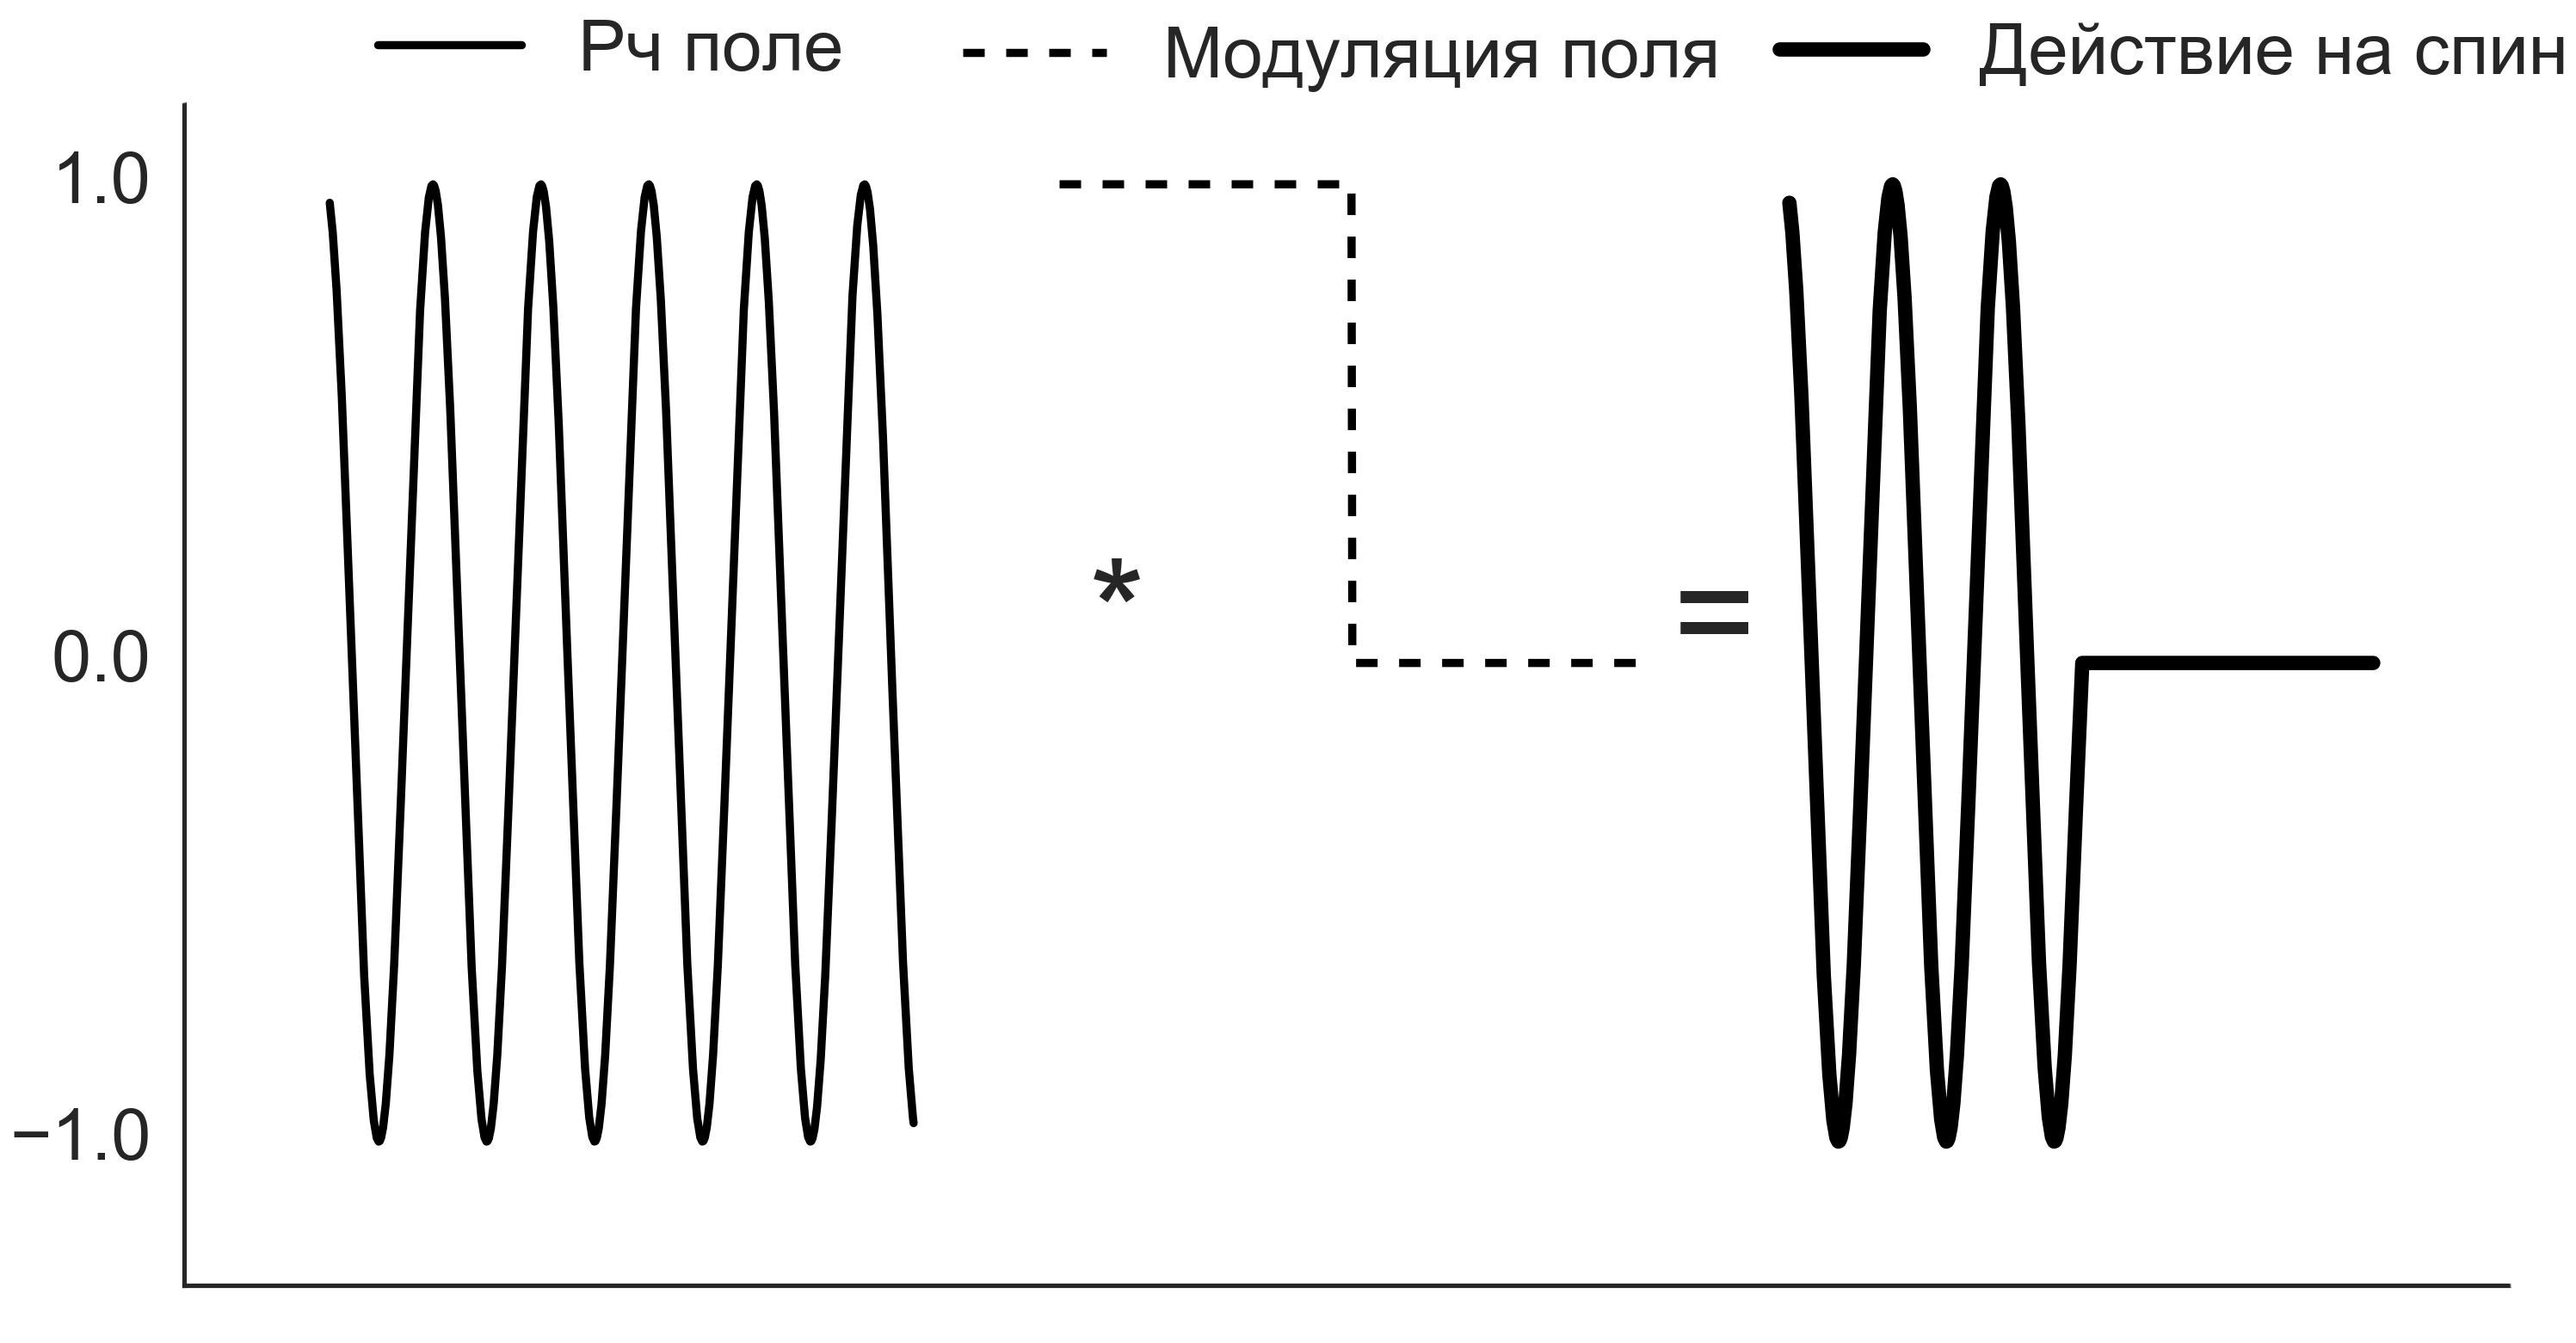
\includegraphics[scale = 0.35]{modulation_rf.png}
	\caption{\textit{Модулированный сигнал, воздействующий на образец - композиция синусоидального рч поля и задающей ступенчатой модуляции}}
	\label{fig:modulation_rf}
\end{figure}

Так, измеряемый сигнал пропорционален разности поляризаций спина в присутствии поля и без него.

При варьировании частоты рч-поля мы получаем узкий резонанс, ширина которого соответствует времени спиновой когерентности $T_2$. Так как к приложенному рч-полю применена модуляция с частотой $f_{mod}$, мы наблюдаем резонансные пики на частотах $f_o \pm m*f_{mod}$, однако, так как форма модуляции во временном представлении ступенчатая, для получения формы модуляции в частотном представлении, нужно произвести преобразование Фурье сигнала, действующего на спин. 

Если представить модулированный сигнал $M_t$

$$M_t = \sin\left( {\omega t}\right) \Theta\left( t\right) $$
где на рис. \ref{fig:modulation_rf}

$$
\Theta (t) = \left\{
\begin{array}
[c]{ll}%
1, t \in \left( \frac{\pi m}{f_m} ; \frac{\pi \left( m + 1 \right) }{f_m} \right) \\
0, t \in \left( \frac{\pi \left( m + 1 \right) }{f_m} ; \frac{\pi \left( m + 2 \right) }{f_m} \right)
\end{array}
\right\}
m \in \mathcal{Z} 
$$

\begin{eqnarray}\label{fourier}
\hat{M_{\omega}} = \int_{0}^{\infty} \sin\left( {\omega t}\right) \Theta\left( t\right) e^{-i \omega t}\,dt = \sum_{m = 0}^{\infty}\int_{\frac{\pi m}{f_m}}^{\frac{\pi \left( m + 1 \right) }{f_m}} \sin\left( {\omega t}\right) e^{-i \omega t}\,dt = \sum_{m = 0}^{\infty}\int_{\frac{\pi m}{f_m}}^{\frac{\pi \left( m + 1 \right) }{f_m}} \sin\left( {\omega t}\right) \left( \cos\left( {\omega t}\right) - i \sin\left( {\omega t}\right)\right)\,dt = \\ = \frac{1}{2 \omega} \sum_{m = 0}^{\infty} e^{- \frac{2 \pi i m \omega}{f_m}} - e^{- \frac{2 \pi i \left( m + 1\right)  \omega}{f_m}} = \frac{ 1 - e^{-\frac{2 \pi i \omega}{f_m}} }{2 \omega} \sum_{m = 0}^{\infty} e^{-\frac{2 \pi i m  \omega}{f_m}}{2 \omega} = \frac{\pi}{f_m} sinc\left( \frac{2 \omega}{f_m} \right)
\end{eqnarray}

\begin{equation}\label{sum}
\sum_{n = 0}^{\infty} \Delta S e^{\frac{-n T_o}{T_2}} \cos{\left( \omega_L n T_o \right) } = Re \sum_{n=0}^{\infty} \Delta S e^{\frac{-n T_o}{T_2}} e^{i \omega_L n T_o} = \Delta S Re\left( \frac{1}{1 - e^{- \frac{T_o}{T_2} + i \omega_L T_o}} \right) = \Delta S Re \left( \frac{1 - e^{- \frac{T_o}{T_2} - i \omega_L T_o}}{1 + e^{-\frac{2 T_o}{T_2}} - 2 e^{-\frac{T_o}{T_2}} \cos{\left( \omega_L T_o \right) }} \right) \approx \\
\end{equation}

$$
\approx \{ \omega_L T_o = 2 \pi k\} \approx \Delta S \frac{1}{1 - e^{-\frac{T_0}{T_2}}} = S
$$

Таким образом, конечный сигнал будет выглядеть следующим образом:

\begin{figure}
	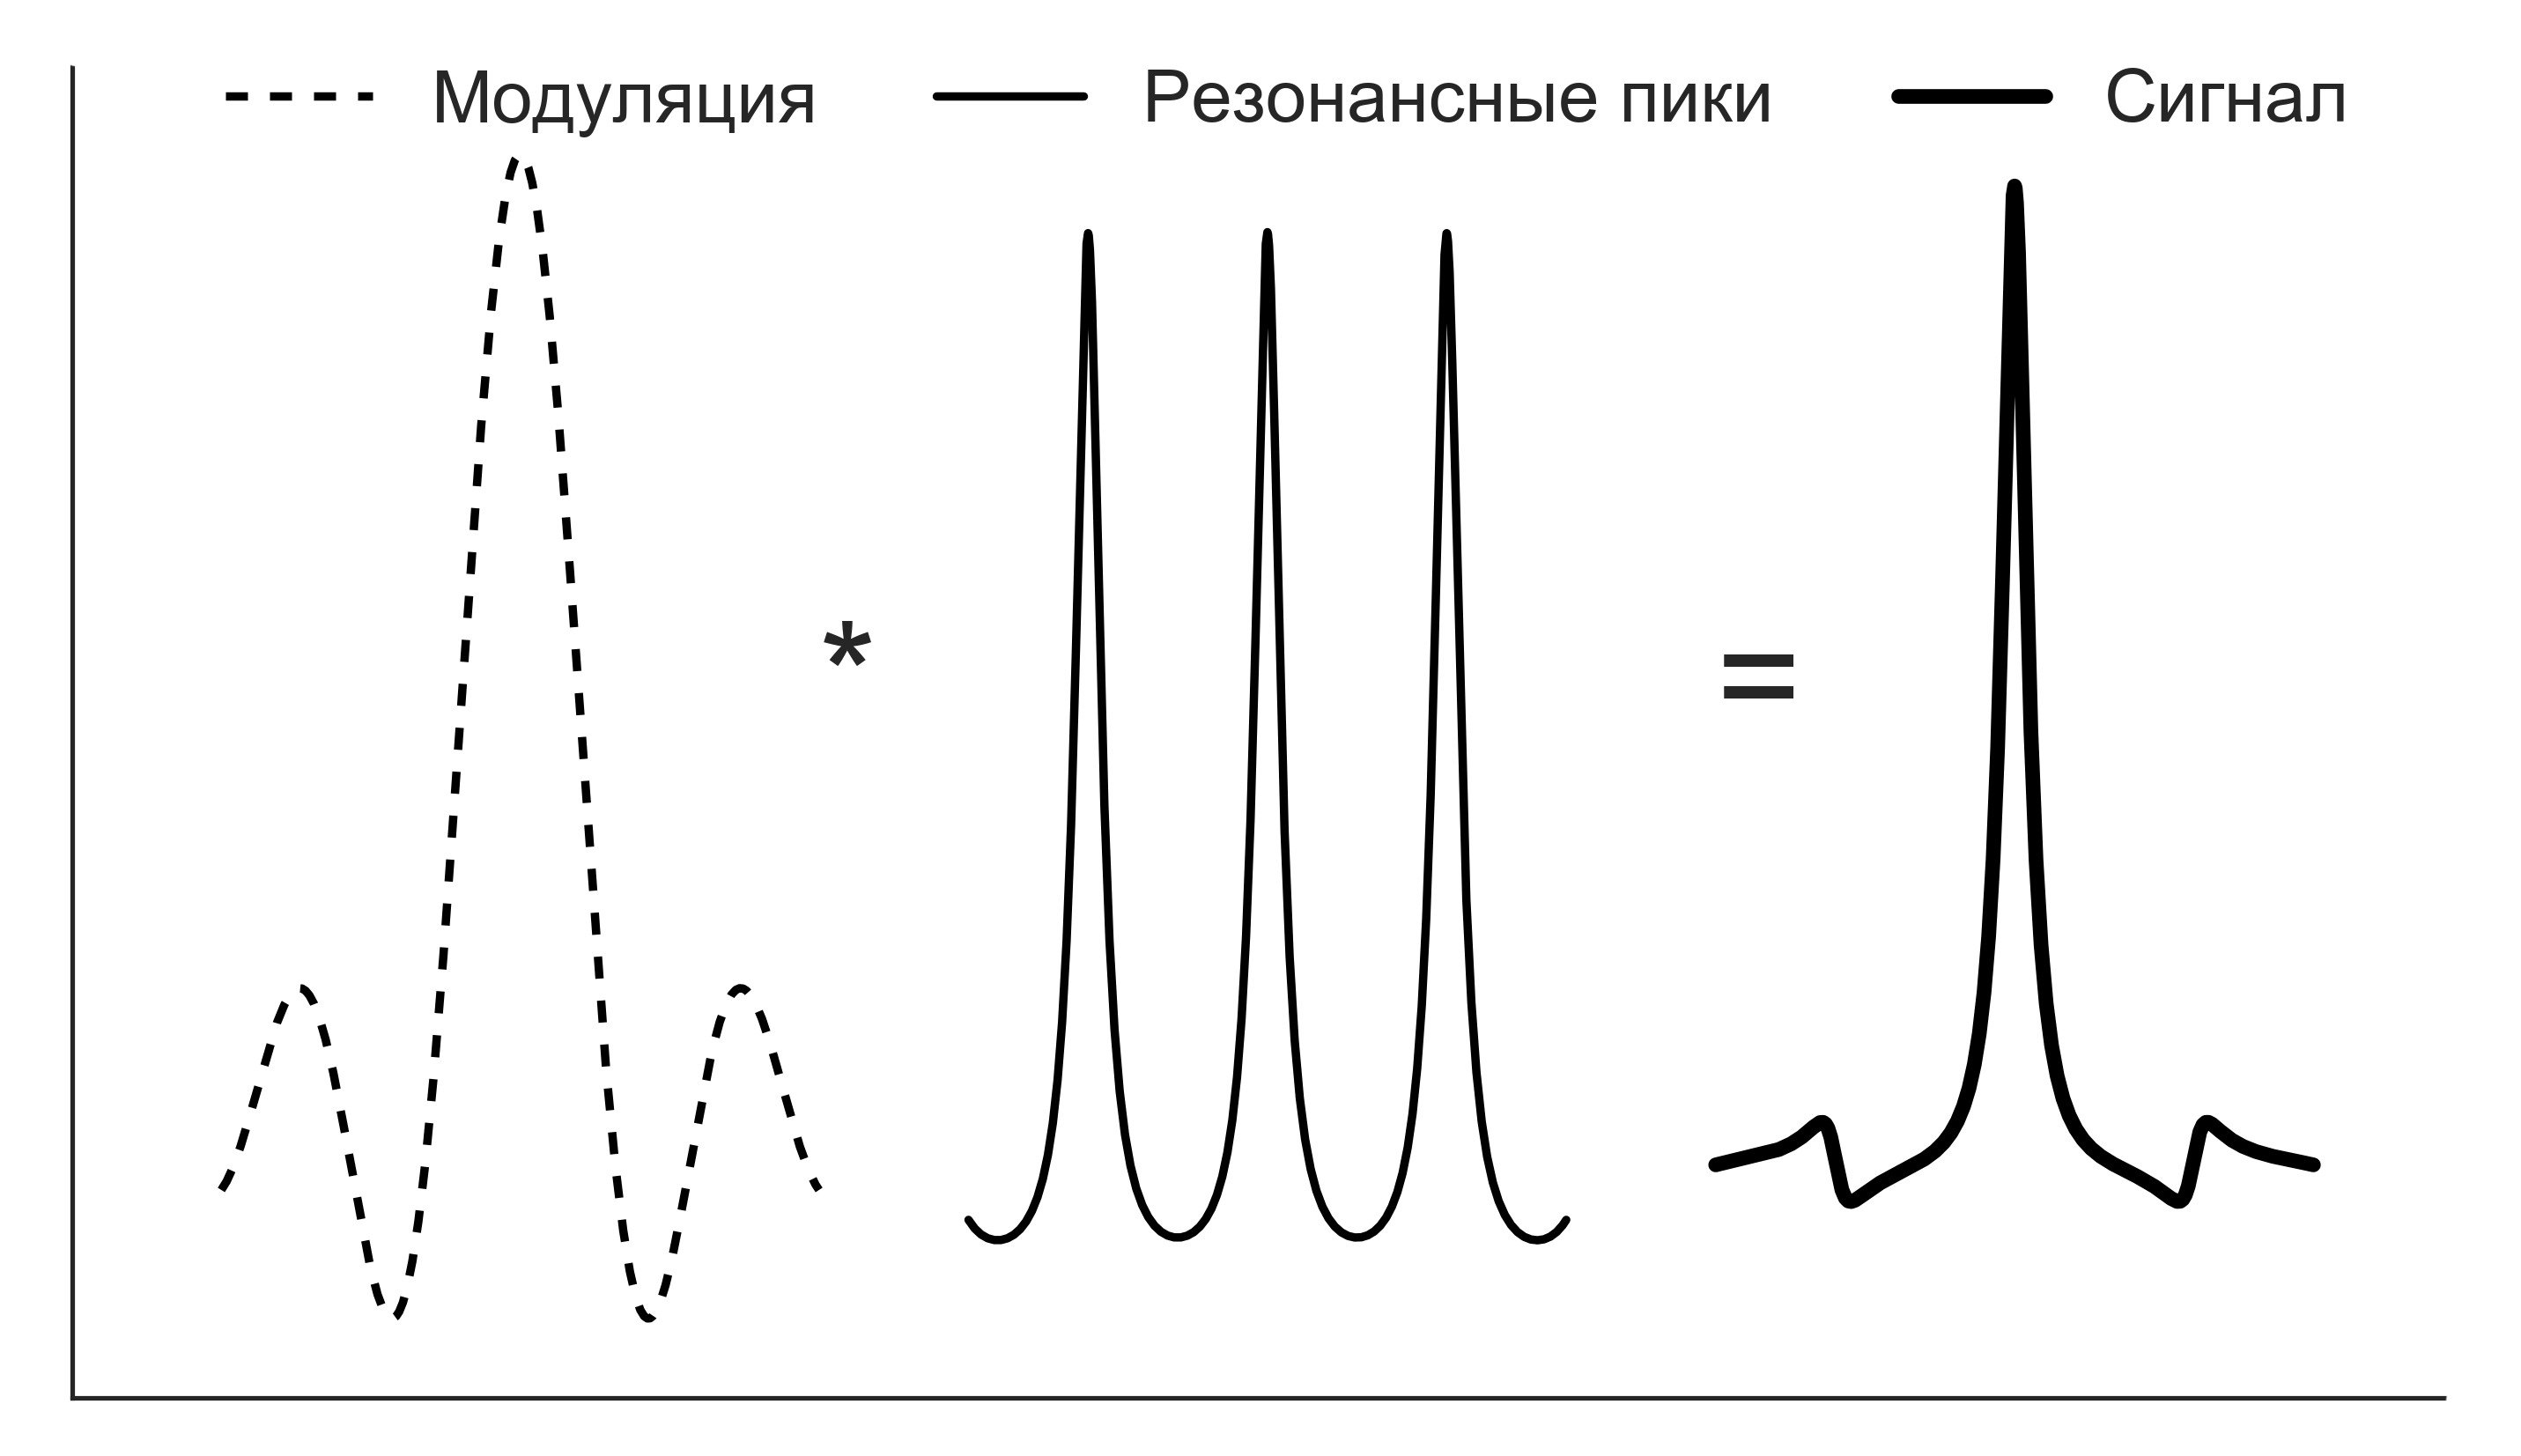
\includegraphics[scale = 0.35]{modulation_graph.png}
	\caption{Итоговый сигнал, состоящий из частотной модуляции с резонансными пиками}
	\label{fig:modulation_graph}
\end{figure}


\begin{thebibliography}{}
	
	\bibitem{dynamics}
	M.W. Wu, J.H. Jiang, M.Q. Weng,
	Spin dynamics in semiconductors, Physics reports, 2010.
	
	\bibitem{mercury}
	A. Kastler, “Optical methods for studying hertzian resonances,” Nobel
	Lecture, 1966
	
	\bibitem{silicium}
	G. Lampel, “Nuclear dynamic polarization by optical electronic saturation
	and optical pumping in semiconductors,” Phys. Rev. Lett., vol. 20, pp. 491–
	493, Mar 1968
	
	\bibitem{spin beats}
	J. J. Baumberg, D. D. Awschalom, N. Samarth, H. Luo, and J. K. Furdyna, Spin beats and dynamical magnetization in quantum structures, Phys. Rev. Lett. 72, 717 (1994)
	
	\bibitem{kikkawa}
	Resonant Spin Amplification in 
	n-Type GaAs
	J. M. Kikkawa and D. D. Awschalom
	Phys. Rev. Lett. 80, 4313 – Published 11 May 1998
	
	\bibitem{flip} 
	P. Siyushev, K. Xia, R. Reuter, M. Jamali, N. Zhao,
	N. Yang, C. Duan, N. Kukharchyk, A. D. Wieck,
	R. Kolesov, and J. Wrachtrup, Coherent properties of single rare-earth spin qubits, Nat. Commun. 5, 3895 (2014).
	
	\bibitem{spin echo}
	E. L. Hahn, Spin echoes, Phys. Rev. 80, 580 (1950).
	
	\bibitem{spin amplification}
	V. V. Belykh, A. R. Korotneva, and D. R. Yakovlev,
	Stimulated resonant spin amplification reveals millisecond electron spin coherence time of rare-earth ions in
	solids, Phys. Rev. Lett. 127, 157401 (2021).
	
	\bibitem{YAG}
	Synthesis and Characterization of YAG: Ce3+ LED Nanophosporos
	Dongdong Jia Y. Wang, X. Guo, K. Li, Y. K. Zou and Weiyi Jia 
	2006 ECS - The Electrochemical Society

\end{thebibliography}

\end{document}